\documentclass[11pt,a4paper,oneside]{article}
\usepackage[latin1]{inputenc}
\usepackage{amsmath}
\usepackage{amsfonts}
\usepackage{amssymb}
\usepackage{graphicx}
\usepackage{color}
\usepackage {tikz}
\usetikzlibrary {er}
\usepackage[left=2.00cm, right=2.00cm, top=1.00cm]{geometry}
\graphicspath{{./}}

\begin{document}
	\title{DS 256 - Scalable Systems for Data Science \\ Assignment 0}
	\author{Shriram R. \\ M Tech (CDS) \\ 06-02-01-10-51-18-1-15763}
	\maketitle
	
	\section{Introduction}
	Analytics of Twitter data has been performed using Apache Spark through its Java interface. The experimental setup, results, plots and analysis are described in detail in the following sections.
     
    \section{Experimental Setup}
    
    \subsection{Hardware}
    Experiments were performed on a commodity cluster having 24 compute nodes. Each node has a 8-core AMD Opteron 3380 processor clocked at 2.6Ghz along with 32GB RAM and 2TB HDD. The nodes are connected through a Gigabit Ethernet switch.
    
    \subsection{HDFS and Spark}
    The HDFS environment has a capacity of 30.93TB with block size 128MB, replication factor of 2 and heartbeat delay of 3s. The global configuration of Spark for all experiments is 4 executors (containers) each having 4 cores and 8GB of memory. The Driver memory was set to 512MB. Apache YARN was used to coordinate the job execution. Experiment specific detail if any is provided below.
    
    \subsection{Dataset}
    The dataset used is a collection of tweets from Twitter between 17th Oct - 16th Dec 2016. The total dataset size is about 955GB and is stored in HDFS by partitioning the dataset into 3984 files of comparable size. Each tweet is described in Twitter Tweet JSON format and is of size approximately 5-10KB . The structure of JSON is described in [1].
     %\begin{center}
     	%\begin{tabular}{|c|c|c|}
     	%	\hline 
     	%	\textbf{Implementation} & \textbf{Insert} & \textbf{Lookup} \\
     	%	\hline
     	%	Hash Table & O(N) & O($\frac{N}{C}$) \\ 
     	%	\hline 
     	%	Unsorted Array & O(N) & O(N)\\ 
     	%	\hline 
     	%	Sorted Array & O(N log N) & O(log N)\\ 
     	%	\hline 
     	%\end{tabular}
     %\end{center}
    -
    \section{Histogram}
    The pseudocode for the histogram of hashtags per tweet is given below,
    \begin{verbatim}
       1. Load all the files into a RDD using Spark textFile()
       2. Parse JSON and emit a tuple <userID, <hashTagCount, 1>> for each valid JSON.
          flatMapToPair transformation is used
       3. Average Hash Tag count is for each user is obtained using a reduceByKey and
          followed by a map transformation
       4. Bucket range and counts are obtained using the histogram transformation
       
       
       
    \end{verbatim}
    The job was executed for the full dataset using the global configuration. Bucket count was chosen arbitrarily as 20 and the result is plotted below,
    
    \begin{center}
    	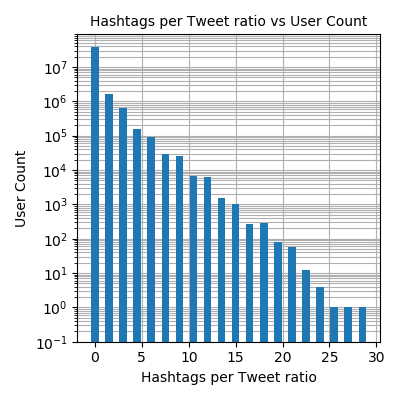
\includegraphics[scale=0.6]{1.png}		
    \end{center}

	It can be observed that the user count decreases as the Hashtag per tweet ratio increases. About 93.5\% of the users fall in the first bucket. The maximum Hashtag per tweet ratio in the given dataset is about 28.5 and the average value is about 0.16.
    
    \section{References}
    \begin{list}{}{}
    	%\item 1. https://en.cppreference.com/
    	\item 2. DS 221 Course lecture notes
    	%\item 3. https://www.geeksforgeeks.org/
    	%\item 4. /home/shriramr/ds221/part\_3/code/test
    	%\item 5. /home/shriramr/ds221/part\_3/data/
    \end{list}
    
\end{document}